\documentclass[tikz,border=10pt]{standalone}
\usepackage{tikz}
\usetikzlibrary{intersections, calc, angles, quotes}

\begin{document}
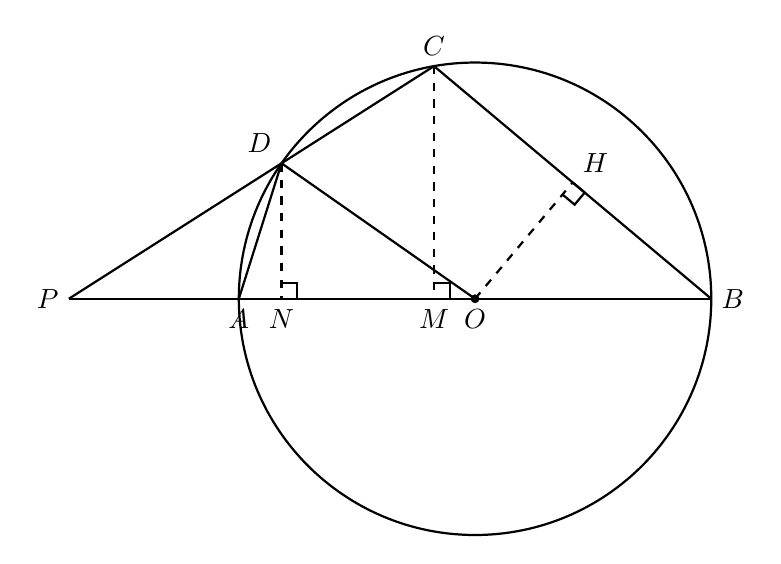
\begin{tikzpicture}[>=stealth, scale=2, thick]

    % 1. 定义基本参数（可根据需要调整半径和角度）
    \def\R{1.5}             % 圆半径
    \def\angC{100}          % 点C的角度
    \def\angD{145}          % 点D的角度
    \coordinate (O) at (0,0);

    % 2. 计算关键点坐标
    \coordinate (A) at (-\R, 0);
    \coordinate (B) at (\R, 0);
    \coordinate (C) at (\angC:\R);
    \coordinate (D) at (\angD:\R);

    % 计算直线 CD 与 BA 延长线的交点 P
    \coordinate (P) at (intersection of C--D and A--B);

    % 计算垂足
    \coordinate (M) at ($(A)!(C)!(B)$); % C 到 AB 的垂足
    \coordinate (N) at ($(A)!(D)!(B)$); % D 到 AB 的垂足
    \coordinate (H) at ($(B)!(O)!(C)$); % O 到 BC 的垂足

    % 3. 绘制几何图形
    \draw (O) circle (\R);              % 绘制圆
    \draw (P) -- (B);                   % 绘制水平轴 PB
    \draw (P) -- (C);                   % 绘制直线 PC (穿过D)
    \draw (C) -- (B);                   % 绘制弦 CB
    \draw (A) -- (D);                   % 绘制弦 AD
    \draw (O) -- (D);                   % 绘制半径 OD

    % 4. 绘制辅助虚线
    \draw[dashed] (C) -- (M);
    \draw[dashed] (D) -- (N);
    \draw[dashed] (O) -- (H);

    % 5. 绘制直角符号
    \draw (M) ++(0, 0.1) -- ++(0.1, 0) -- ++(0, -0.1);
    \draw (N) ++(0, 0.1) -- ++(0.1, 0) -- ++(0, -0.1);
    % H 处的直角符号需要旋转
    \begin{scope}[shift={(H)}, rotate={60-190}]
        \draw (0,0) -- (0,0.1) -- (0.1,0.1) -- (0.1,0);
    \end{scope}

    % 6. 标注点和标签
    \fill (O) circle (0.8pt); % 标注圆心 O
    \node[below] at (O) {$O$};
    \node[below] at (A) {$A$};
    \node[right] at (B) {$B$};
    \node[above] at (C) {$C$};
    \node[above left] at (D) {$D$};
    \node[left] at (P) {$P$};
    \node[below] at (M) {$M$};
    \node[below] at (N) {$N$};
    \node[above right] at (H) {$H$};

\end{tikzpicture}
\end{document}